\documentclass[a4paper,11pt]{article}
\usepackage{color}
\usepackage{pdfpages}
\usepackage{graphicx}
\graphicspath{{./figures/}}
\usepackage{subcaption}
\usepackage{wrapfig}
\usepackage[export]{adjustbox}
\usepackage{geometry}
\usepackage{setspace}
\usepackage{adjustbox}
\usepackage{amsmath}
\usepackage{textgreek}
\usepackage{authblk}
\usepackage[british]{babel}
\usepackage{url}
\usepackage{doi}
\usepackage{siunitx}
\usepackage{textcomp}
\usepackage[utf8]{inputenc}% for appendix
\usepackage{appendix} %for appendix
\usepackage[square,numbers]{natbib} %the big one
\usepackage{titlepic}
\doublespacing
\geometry{legalpaper, portrait, margin=2cm}
\begin{document}
\title{Open Science Hardware Setup for investigating the Stability of Organic Solar Cells - Interim Report}
\author{Samuel Mendis}
\affil{Department of Engineering Science, University of Oxford}
\affil{Department of Physics, University of Oxford}
\date{\today}
\titlepic{
\includegraphics[width=0.3\textwidth]{oxford_logo}}
\maketitle
\pagebreak
\section{Introduction}
Solar cells are becoming increasingly prevalent in the fight against climate change\cite[p.~34]{RN49}, leading demand to increase worldwide. This project aims to contribute to the development of the next generation of solar cells to be manufactured out of carbon-based materials (rather than the current industry standard of silicon). Currently, controlled lifetime testing of organic solar cells is difficult due to the multitude of failure mechanisms. These are caused by chemical degradation via oxygen and water\cite[p.~689]{RN38}. To combat this problem, this project will design, manufacture and test a well controlled lifetime solar testing container. This project is being run in conjunction with the Advanced Functional Materials and Devices group (AFMD) in the department of Physics, headed by Professor Moritz Riede. Therefore I am, and will be collaborating closely with the members of AFMD to ensure the device meets the specification they require. A key tenet of the project is ensuring the accessibility of the research through the use of open hardware in order for the  potential acceleration of the development of organic solar cells.
\section{Aims and Objectives}
The aim of the container is to simulate a lifetime (for example: 20 years) of real world degradation in a \emph{reasonable} timeframe. Reasonable means that ideally the testing container should be able to test the solar cell in a short cycle test (15 minutes) or a long multiple cycle test (up to 3 months). To ensure accurate testing of the cells, the container needs to be airtight. This is to prevent any uncontrolled variables from entering the testing container and causing degradation of the cell. Furthermore, the container should have to have gas inlets and outlets so that the conditions that the solar cell is tested under can be varied in a controlled manner. This will be in conjunction with a temperature controller capable of varying the temperature of the solar cell up to 120\textdegree C. These objectives were guided by the paper \emph{Consensus stability testing protocols for organic photovoltaic materials and devices} \cite[p.~1255-1261]{RN47} which cites multiple different testing criteria for an organic solar cell - in the absence of a tailored ISO standard. Additional aims that would enhance the scope of the project is a graphical user interface (GUI) developed to control the conditions within the testing container. To ensure the project is completed, not all the components will be manufactured from scratch, some will be purchased while others are provided by the AFMD research group and existing open science hardware/software efforts. Some of the components include: the push-fit valves, a safety relief valve, o-rings, a mass flow controller and an illumination source.

\section{Progress}
At this stage in the year, the container is past the design stage and is onto manufacturing, with the outer shell being manufactured within the Engineering Science Workshop from AL-xxxx. A full design was completed using the open source software OpenSCAD. Using inspiration from Karl-Augustin Zaininger (a Physics researcher who has developed a similar type of device, without the functionality) a CAD model of the testing container was built and is shown in Figure \ref{fig:model}.The outer shell (coloured in green) is the component currently bring manufactured. The red circular parts will be 3D printed using acrylic and will be used to hold metal pins to connect a controller on the outside to the instrumentation within.  \\ 
\begin{figure}[h]
\begin{subfigure}{0.5\textwidth}
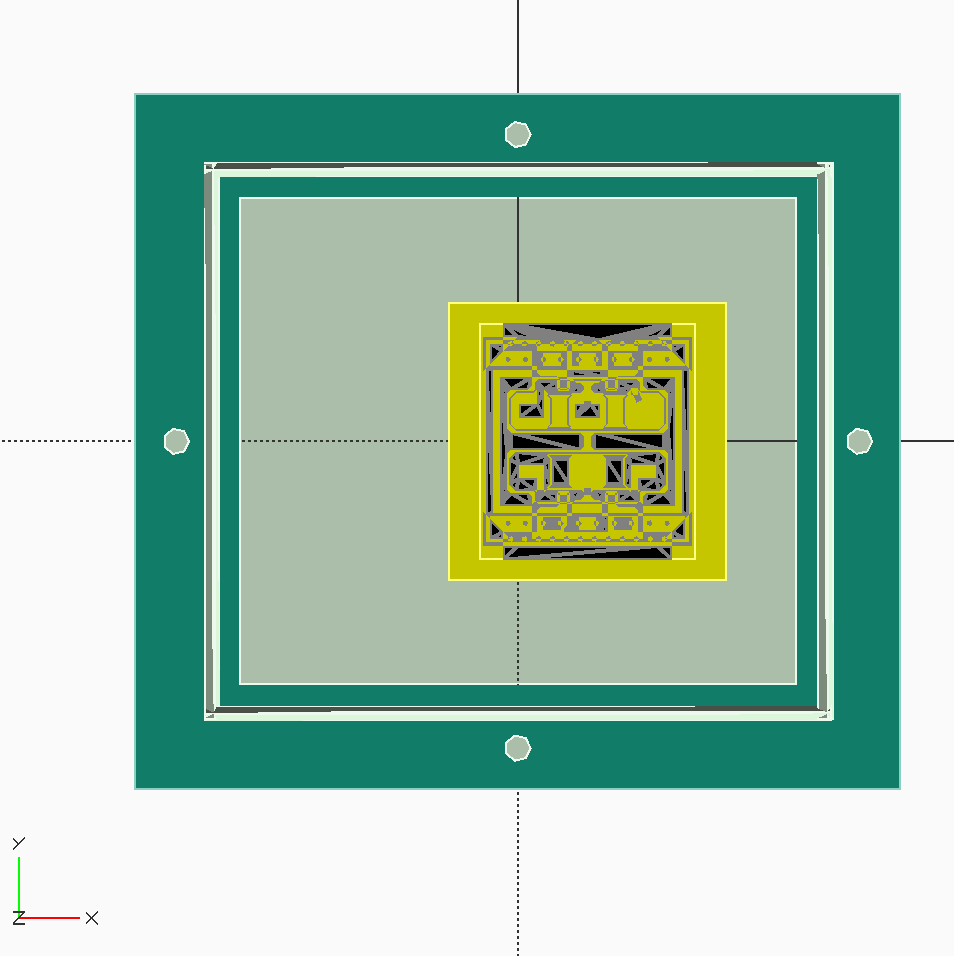
\includegraphics[width=0.8\linewidth]{fig1a}
\caption{Plan View of Model}
\label{fig:subim1}
\end{subfigure} \begin{subfigure}{0.5\textwidth}
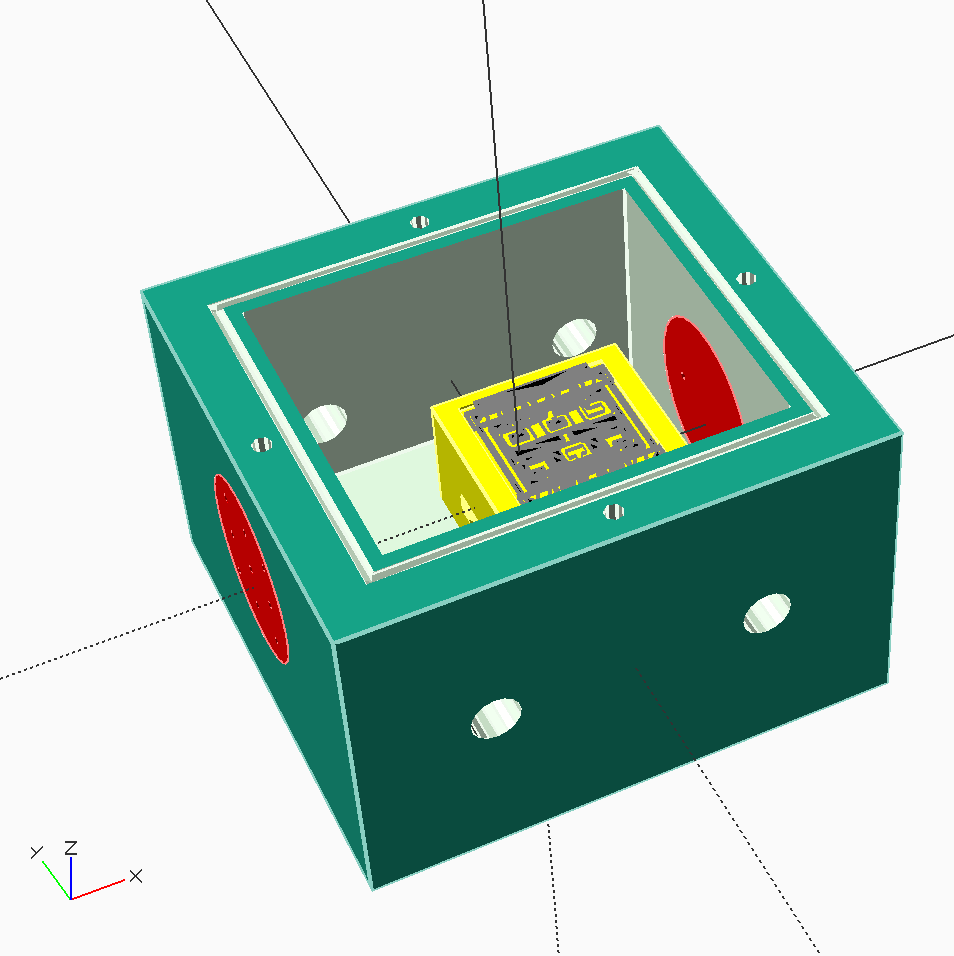
\includegraphics[width=0.8\linewidth]{fig1b}
\caption{Isometric View of Model}
\label{fig:subim2}
\end{subfigure}
\caption{Showing plan and isometric view of the full OpenSCAD model\label{fig:model}}
\label{fig:image2}
\end{figure}
\noindent The three important factors that the container had to accommodate were: the substrate (shown in black in Figure \ref{fig:model}), any electronic devices (e.g. a temperature controller)  and gas inlet ports. The substrate used carries 6 solar cells with dimensions of 30 mm x 30 mm and a thickness of 1.1 mm. The substrate design in Figure \ref{fig:model} was provided to me by Dr Grey Christophoro - Physics researcher \cite{RN48}. In order to carry the substrate in the testing container, a substrate holder (coloured yellow in Figure \ref{fig:model}) was designed to fit within the outer shell of the box. The modular design is deliberate to allow the user to modify which cells and layouts are being tested, without the redesign of the entire container, just the substrate holder; thereby saving those who may need to use it in the future valuable time and money. 
\section{Future Work}
During the manufacturing of the box, there is an opportunity to start on simulations of the heat and mass flow within the container. These simulations will be conducted using SOLIDWORKS flow and heat simulations features to provide a more accurate picture of the environmental variation around the substrate. These simulations will allow the user to control the environment with a better understanding, hence creating more consistent ageing conditions. Once the outer shell has been manufactured, following key steps are to pressure test the vessel, implement the control electronics, calibrate the temperature and environmental sensors as well as installing the container in front of a lamp. Once the calibration is complete the container will be assessed in known control environments to check whether the solar cells output as predicted. The Gantt chart (shown in the Appendix) shows the full outline of the future plans including contingency time at the end of Hilary term. 
\begin{singlespace}
\bibliographystyle{unsrtnat} %also the big one 
\bibliography{mtreport1}
\end{singlespace}

\appendix
\appendixpage
\begin{appendix}
\includegraphics[width=1.7\linewidth, angle=270]{gantt}
\end{appendix}

\end{document}